\RequirePackage[T1]{fontenc}   % before the class, so IEEEtran's Times (ptm) loads in T1
\documentclass[conference]{IEEEtran}
\IEEEoverridecommandlockouts
\usepackage[utf8]{inputenc}
\renewcommand{\ttdefault}{lmtt}   % Latin Modern Typewriter for code-like names
\usepackage[spanish,es-nodecimaldot,es-tabla,es-noshorthands]{babel}
\usepackage{cite}
\usepackage{amsmath,amssymb}
\usepackage{graphicx}
\usepackage{booktabs}
\usepackage{array}
\usepackage{textcomp}
\usepackage{xcolor}
\usepackage{microtype}
\usepackage[hidelinks]{hyperref}
\usepackage{url}
\def\UrlBreaks{\do\_\do\.\do\/\do\-}

\newcommand{\x}{\ensuremath{\times}}
\newcolumntype{L}[1]{>{\raggedright\arraybackslash}p{#1}}
\renewcommand{\figurename}{Figura}
\renewcommand{\IEEEkeywordsname}{Palabras clave}

\begin{document}

\title{Más agentes, más costo: evaluación costo--calidad de topologías de \textit{swarms} de agentes LLM con un orquestador agnóstico al modelo y al dominio
\thanks{Paper, curso Inteligencia Artificial (G1), Universidad Icesi, Cali, Colombia. Fecha: 7 de octubre de 2026.}}

\author{\IEEEauthorblockN{Julián Andrés Mendoza Castro}
\IEEEauthorblockA{Código A00395237\\
Universidad Icesi\\
Cali, Colombia\\
1109185879@u.icesi.edu.co}
\and
\IEEEauthorblockN{Esteban Gaviria Zambrano}
\IEEEauthorblockA{Código A00396019\\
Universidad Icesi\\
Cali, Colombia\\
esteban.gaviria@u.icesi.edu.co}}

\maketitle

\begin{abstract}
Un \textit{swarm} de agentes LLM reparte una tarea entre varios agentes que se comunican, pero cada agente y cada mensaje se pagan en tokens. Este trabajo presenta un orquestador reina--obreros que cambia de modelo y de dominio solo con configuración, y lo usa para medir de forma controlada cuánto cuesta y cuánto aporta coordinar. Se comparan el agente único, una topología jerárquica y una malla con $n=2$ y $n=4$ obreros, sobre \texttt{deepseek-flash} sin razonamiento extendido, en tres dominios: GSM8K-Platinum, problemas de nivel 5 de MATH-500 y la planificación de un viaje a Cartagena. Se registró el uso real de la API en 195 corridas (921 llamadas, 0 fallos técnicos) por USD~0.22. Ninguna configuración superó al agente único en calidad: las dos tareas matemáticas quedaron en el techo (exactitud 1.00 en todas las configuraciones) y en la rúbrica de Cartagena el agente único obtuvo 1.00 frente a 0.81--1.00 de los \textit{swarms}. El costo por corrida, en cambio, creció entre 2.7\x{} y 16.6\x{} respecto al agente único, y al pasar de 2 a 4 obreros la malla creció entre 2.4 y 3.8 veces más rápido que la jerárquica, porque su ronda de revisión escala con $n^2$. Las mismas corridas muestran que la redundancia sí corrige errores internos (en MATH, la revisión de la malla corrigió a todos los obreros equivocados), pero sobre tareas que un solo agente ya resuelve esa corrección no se traduce en calidad final. Dos modelos locales de 3B en Ollama ejecutaron el mismo código como prueba de portabilidad.
\end{abstract}

\begin{IEEEkeywords}
Sistemas multiagente, modelos de lenguaje, orquestación, topologías de comunicación, costo--calidad, modos de fallo.
\end{IEEEkeywords}

\section{Introducción}

Los sistemas multiagente basados en LLM asignan roles a varios agentes que conversan para resolver una tarea \cite{guo2024survey}. AutoGen los modela como conversaciones programables \cite{wu2024autogen}, GPTSwarm como grafos cuyos nodos y aristas se pueden optimizar \cite{zhuge2024gptswarm}, y herramientas como Ruflo los ofrecen como \textit{swarms} con una reina y obreros \cite{ruflo}. Coordinar tiene un costo directo: Anthropic reporta que su sistema de investigación multiagente usa unas 15 veces los tokens de un chat \cite{anthropic2025multiagent}. También tiene un costo de fiabilidad: la taxonomía MAST atribuye la mayoría de los fallos de estos sistemas al diseño y a la coordinación, no al modelo \cite{cemri2025mast}, y un estudio reciente encontró que, cuando el agente único ya resuelve más del 45\,\% de una tarea, agregar agentes da retornos negativos \cite{kim2025scaling}.

La pregunta de este trabajo es la que plantea la retroalimentación del curso: \emph{¿agregar agentes y comunicación mejora la calidad lo suficiente para justificar el aumento de costo?} Para responderla con la misma vara se necesita que todo lo demás quede fijo: el modelo, los \textit{prompts}, los límites de generación y la evaluación. Las contribuciones son tres:
\begin{itemize}
\item Un orquestador reina--obreros en Python, agnóstico al modelo (la misma API sirve para DeepSeek y para modelos locales en Ollama) y al dominio (cada dominio es un conjunto de datos: roles, tareas, formatos y métrica), publicado con todos sus datos \cite{repo2026swarm}.
\item Una comparación controlada de costo y calidad de tres topologías con $n\in\{2,4\}$ en tres dominios, con el uso real de tokens que reporta la API, costo, latencia, fallos y señales de coordinación.
\item Hallazgos metodológicos que afectan a cualquier réplica: una etiqueta errónea de GSM8K, el truncamiento silencioso del contexto en Ollama y la discrepancia entre un juez LLM y la rúbrica.
\end{itemize}

\section{Trabajo relacionado}

La Tabla~\ref{tab:rel} ubica este trabajo frente a los artículos base y a los estudios de escalamiento. AutoGen reportó que su conversación multiagente supera a GPT-4 solo en el conjunto completo de MATH (69.48\,\% frente a 55.18\,\%) \cite{wu2024autogen}. GPTSwarm optimiza las aristas del grafo, y AgentPrune muestra que muchas son redundantes: podarlas reduce entre 28.1\,\% y 72.8\,\% de los tokens con resultados comparables \cite{zhang2025agentprune}. MacNet escala colaboraciones a más de mil agentes en grafos acíclicos \cite{qian2025macnet}, y el muestreo con votación mejora con el número de agentes \cite{li2024moreagents}. En sentido contrario, Kim et~al.~\cite{kim2025scaling} miden que los sistemas centralizados amplifican los errores 4.4\x{} y los descentralizados 7.8\x{} respecto al agente único, y los errores de modelos distintos están correlacionados \cite{kim2025correlated}, lo que debilita la premisa de independencia del voto. Kapoor et~al.~\cite{kapoor2024agents} piden comparar agentes siempre contra su costo y con frentes de Pareto. Este trabajo sigue esa recomendación con topologías fijas, sin optimizarlas.

\begin{table}[t]
\centering
\caption{Trabajos relacionados y lo que mide cada uno}
\label{tab:rel}
\footnotesize
\setlength{\tabcolsep}{3pt}
\begin{tabular}{@{}L{1.9cm}L{2.5cm}L{3.5cm}@{}}
\toprule
Trabajo & Organización & Qué mide \\
\midrule
AutoGen \cite{wu2024autogen} & conversación entre agentes & exactitud (MATH, otras) \\
GPTSwarm \cite{zhuge2024gptswarm} & grafo optimizable & exactitud y costo de optimizar \\
AgentPrune \cite{zhang2025agentprune} & poda de aristas & tokens frente a exactitud \\
MAST \cite{cemri2025mast} & 7 marcos existentes & 14 modos de fallo \\
Kim et~al. \cite{kim2025scaling} & 5 arquitecturas & escalamiento y amplificación de errores \\
Este trabajo & único, jerárquica, malla & costo real, calidad, latencia y fallos al variar $n$ \\
\bottomrule
\end{tabular}
\end{table}

\section{Metodología}

\subsection{Orquestador}

Un agente es un rol, unas instrucciones y un acceso a un LLM a través de una interfaz única, \texttt{LLM.complete()}, que oculta el proveedor. Las tres topologías (Fig.~\ref{fig:topo}) comparten las etapas:
\begin{enumerate}
\item \textbf{Plan.} La reina reparte la tarea y devuelve una lista JSON con una subtarea por obrero. Si el JSON es inválido o no asigna exactamente una subtarea a cada obrero, se registra el fallo y cada obrero recibe la tarea completa.
\item \textbf{Trabajo.} Cada obrero resuelve su subtarea.
\item \textbf{Revisión} (solo malla). Cada obrero lee los borradores de todos y revisa el suyo.
\item \textbf{Integración.} La reina combina las contribuciones en la respuesta final.
\end{enumerate}
El agente único responde directamente con el mismo formato final. Los obreros de los dominios matemáticos cierran con una línea \texttt{\#\#\#\# <número>}, lo que permite saber si algún obrero tenía la respuesta correcta y si la reina la conservó.

\begin{figure}[t]
\centering
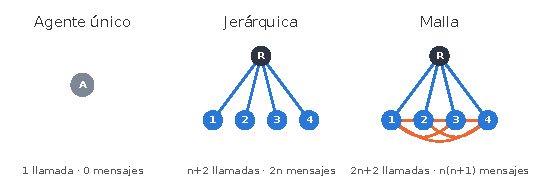
\includegraphics[width=\columnwidth]{figs/topologias.pdf}
\caption{Topologías comparadas con $n=4$ obreros. R es la reina; en la malla, las aristas naranjas son la ronda de revisión entre obreros.}
\label{fig:topo}
\end{figure}

\subsection{Modelo de costo}

Con $n$ obreros, la jerárquica hace $n+2$ llamadas e intercambia $2n$ mensajes; la malla hace $2n+2$ llamadas y $n(n+1)$ mensajes. El costo de una corrida es
\begin{equation}
C=\sum_{k\in\text{llamadas}}\left(t^{\text{in}}_k\,p^{\text{in}}+t^{\text{out}}_k\,p^{\text{out}}\right),
\label{eq:cost}
\end{equation}
con los tokens $t$ que reporta la API y los precios de lista de \texttt{deepseek-flash} consultados el 7 de octubre de 2026: $p^{\text{in}}=0.30$ y $p^{\text{out}}=1.20$ USD por millón de tokens \cite{deepseek2026pricing}. Se usa el precio de lista (pico, sin caché) para comparar configuraciones, porque el precio facturado depende de la hora del día y de lo que ya estuviera en caché. Si cada borrador mide $w$ tokens y el resto del \textit{prompt} $b$, la integración lee $b+nw$ tokens, mientras que la revisión hace $n$ llamadas de $b+nw$ tokens cada una:
\begin{equation}
t^{\text{in}}_{\text{rev}}\approx n\,b+n^2 w ,
\label{eq:rev}
\end{equation}
de modo que el costo de la malla crece de forma cuadrática, no exponencial, con $n$.

\subsection{Dominios}

Cada dominio es un conjunto de datos y la Tabla~\ref{tab:dom} los resume. GSM8K-Platinum es la partición de prueba de GSM8K \cite{cobbe2021gsm8k} con las etiquetas erróneas corregidas \cite{vendrow2025platinum}. MATH-500 \cite{lightman2024verify} es un subconjunto del conjunto de prueba de MATH \cite{hendrycks2021math}; se tomaron solo problemas de nivel 5 con respuesta entera para mantener la coincidencia exacta. Este dominio se agregó después de observar el techo en GSM8K, así que su hipótesis es \textit{post hoc}. La tarea abierta es el caso de Cartagena propuesto en la presentación del curso: un viaje de 3 días para un estudiante con 600\,000 COP y alojamiento económico.

\begin{table}[t]
\centering
\caption{Dominios, tareas y medida de calidad}
\label{tab:dom}
\footnotesize
\setlength{\tabcolsep}{3pt}
\begin{tabular}{@{}L{1.75cm}L{3.4cm}L{2.75cm}@{}}
\toprule
Dominio & Tareas (semilla fija) & Calidad \\
\midrule
GSM8K-Platinum & 10 problemas de aritmética escolar & coincidencia exacta \\
MATH-500 niv.~5 & 10 de 74 problemas con respuesta entera & coincidencia exacta \\
Cartagena & 1 plan de viaje abierto & rúbrica binaria de 7 criterios \\
\bottomrule
\end{tabular}
\end{table}

\subsection{Protocolo}

El experimento principal usa \texttt{deepseek-flash} (DeepSeek-V4.1-Flash) a través de la API oficial, con el razonamiento extendido desactivado; ninguna llamada generó tokens de razonamiento. Todas las configuraciones comparten temperatura 0.7, un máximo de 2\,048 tokens de salida y los mismos \textit{prompts}. Un piloto con 1\,024 tokens truncó dos de seis llamadas de la malla en Cartagena, por lo que se descartó y se subió el límite. Repeticiones: en GSM8K, 3 muestras del agente único y 2 de cada \textit{swarm} por problema; en MATH, 3 y 1, porque 2 repeticiones no cabían en el presupuesto; en Cartagena, 3 por configuración. Cada corrida tiene un identificador derivado de su especificación, se ejecuta en orden aleatorio con semilla fija (cuatro a la vez) y queda registrada con cada una de sus llamadas. Un tope de gasto de USD~0.50 detenía la ejecución si el gasto más la proyección del resto lo superaba.

\subsection{Evaluación}

En los dominios matemáticos la calidad es la coincidencia exacta del número final, sin juez LLM. Cartagena se califica con una rúbrica de siete criterios binarios con reglas de decisión explícitas (itinerario por día, presupuesto con total, total dentro del límite, alojamiento económico, dos riesgos con mitigación, consistencia interna y lugares concretos). Las 15 respuestas se exportaron sin modelo ni arquitectura, en orden aleatorio, y las calificó a ciegas un evaluador LLM distinto del generador (Claude Opus 5.5) antes de abrir la clave; \textbf{no es una evaluación humana}. Como análisis secundario, el propio \texttt{deepseek-flash} actuó como juez, lo que introduce sesgo de autopreferencia \cite{panickssery2024selfpref,zheng2023judging}. Se registran fallos técnicos (error, \textit{timeout}, plan inválido, formato, truncamiento de la salida o del contexto) y, en los dominios matemáticos, si algún obrero acertó, si la reina conservó o perdió la respuesta correcta y si la revisión de la malla mejoró o empeoró a los obreros. Las comparaciones usan intervalos \textit{bootstrap} al 95\,\% y la prueba exacta de McNemar \cite{mcnemar1947} sobre los mismos problemas.

\section{Resultados}

\subsection{Costo}

La Tabla~\ref{tab:main} resume las 195 corridas. Las llamadas y los mensajes coincidieron exactamente con las fórmulas en todas las corridas. Frente al agente único, el costo por corrida a precio de lista fue de 2.7\x{} a 8.8\x{} en la jerárquica y de 4.0\x{} a 16.6\x{} en la malla (Fig.~\ref{fig:cost}). De $n=2$ a $n=4$, la jerárquica sumó entre 1.9 y 3.7 veces el costo del agente único, y la malla entre 5.4 y 8.9 veces. La Fig.~\ref{fig:stage} muestra de dónde sale esa diferencia: con $n=4$, la ronda de revisión concentra el 55\,\% de los tokens de la malla en GSM8K, el 69\,\% en MATH y el 64\,\% en Cartagena, como predice la ec.~\eqref{eq:rev}. La latencia, medida solo dentro de la API, creció de 2.3\x{} a 10.4\x{}, porque las llamadas de una corrida son secuenciales. El \textit{prompt} más largo fue de 8\,129 tokens (MATH, malla con $n=4$, revisión).

\begin{table*}[t]
\centering
\caption{Resultados por dominio y configuración (\texttt{deepseek-flash}). Calidad con IC \textit{bootstrap} al 95\,\%; costo a precio de lista en milésimas de USD por corrida; ``\x'' es el cociente frente al agente único del mismo dominio.}
\label{tab:main}
\footnotesize
\setlength{\tabcolsep}{4.2pt}
\begin{tabular}{@{}llrcrrrrrrrr@{}}
\toprule
Dominio & Config. & Corridas & Calidad [IC 95\,\%] & Llamadas & Mensajes & Tokens & \x & Costo (mUSD) & \x & Latencia (s) & \x \\
\midrule
GSM8K-Platinum & único  & 30 & 1.00 [1.00, 1.00] & 1  & 0  & 178    & 1.0  & 0.12  & 1.0  & 1.3  & 1.0  \\
               & jer-2  & 20 & 1.00 [1.00, 1.00] & 4  & 4  & 1\,072 & 6.0  & 0.61  & 5.1  & 5.2  & 4.1  \\
               & jer-4  & 20 & 1.00 [1.00, 1.00] & 6  & 8  & 1\,818 & 10.2 & 1.06  & 8.8  & 8.2  & 6.5  \\
               & malla-2 & 20 & 1.00 [1.00, 1.00] & 6  & 6  & 1\,736 & 9.7  & 0.93  & 7.7  & 7.8  & 6.2  \\
               & malla-4 & 20 & 1.00 [1.00, 1.00] & 10 & 20 & 4\,005 & 22.5 & 2.00  & 16.6 & 13.2 & 10.4 \\
\midrule
MATH-500 niv.~5 & único  & 30 & 1.00 [1.00, 1.00] & 1  & 0  & 864     & 1.0  & 0.92 & 1.0 & 4.1  & 1.0 \\
                & jer-2  & 10 & 1.00 [1.00, 1.00] & 4  & 4  & 3\,518  & 4.1  & 2.46 & 2.7 & 9.5  & 2.3 \\
                & jer-4  & 10 & 1.00 [1.00, 1.00] & 6  & 8  & 5\,980  & 6.9  & 4.20 & 4.6 & 16.1 & 3.9 \\
                & malla-2 & 10 & 1.00 [1.00, 1.00] & 6  & 6  & 6\,019  & 7.0  & 3.68 & 4.0 & 13.1 & 3.2 \\
                & malla-4 & 10 & 1.00 [1.00, 1.00] & 10 & 20 & 16\,763 & 19.4 & 8.68 & 9.4 & 25.3 & 6.1 \\
\midrule
Cartagena & único  & 3 & 1.00 [1.00, 1.00] & 1  & 0  & 879     & 1.0  & 0.98  & 1.0  & 6.2  & 1.0 \\
          & jer-2  & 3 & 0.81 [0.71, 0.86] & 4  & 4  & 4\,198  & 4.8  & 3.39  & 3.5  & 15.7 & 2.5 \\
          & jer-4  & 3 & 1.00 [1.00, 1.00] & 6  & 8  & 6\,944  & 7.9  & 5.37  & 5.5  & 27.5 & 4.5 \\
          & malla-2 & 3 & 0.95 [0.86, 1.00] & 6  & 6  & 9\,645  & 11.0 & 6.79  & 7.0  & 27.8 & 4.5 \\
          & malla-4 & 3 & 1.00 [1.00, 1.00] & 10 & 20 & 23\,750 & 27.0 & 14.13 & 14.5 & 50.9 & 8.3 \\
\bottomrule
\end{tabular}
\end{table*}

\begin{figure*}[t]
\centering
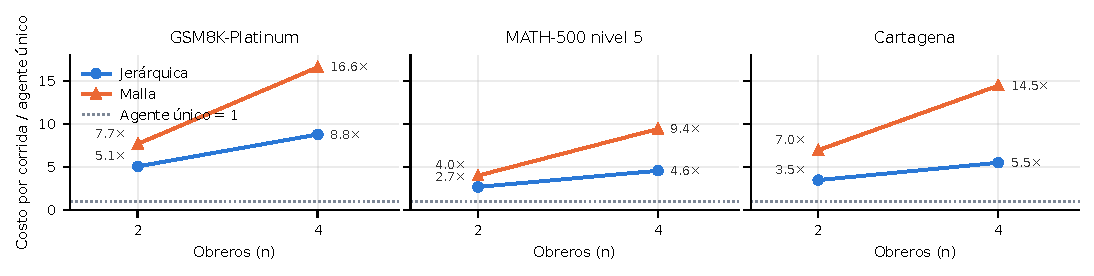
\includegraphics[width=\textwidth]{figs/costo_vs_n.pdf}
\caption{Costo por corrida relativo al agente único al pasar de $n=2$ a $n=4$ obreros. En los tres dominios, la malla crece más del doble de rápido que la jerárquica.}
\label{fig:cost}
\end{figure*}

\begin{figure*}[t]
\centering
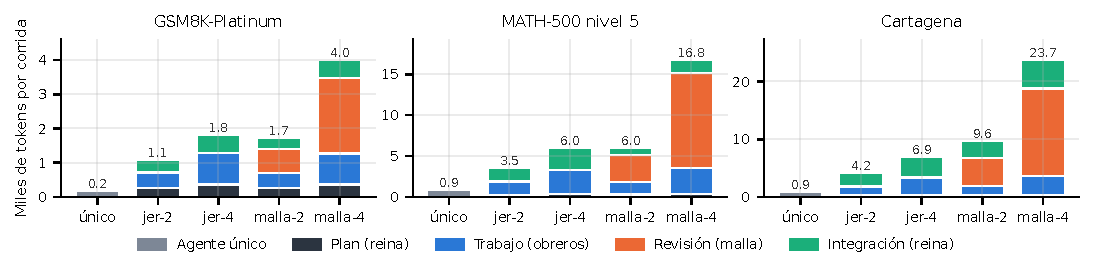
\includegraphics[width=\textwidth]{figs/tokens_por_etapa.pdf}
\caption{Tokens promedio por corrida según la etapa. La revisión de la malla domina el costo con $n=4$.}
\label{fig:stage}
\end{figure*}

\subsection{Calidad}

El agente único resolvió los 10 problemas de GSM8K-Platinum y los 10 de MATH en sus 30 muestras de cada dominio, y lo mismo hicieron las 80 y 40 corridas de \textit{swarm}. Con ambos dominios en el techo no hay pares discordantes para McNemar ni margen para que la coordinación mejore el resultado. En Cartagena, la rúbrica dio 1.00 al agente único y a jer-4 y malla-4, 0.95 a malla-2 y 0.81 a jer-2, la única diferencia con un intervalo que excluye el cero (de $-0.29$ a $-0.14$ en tres repeticiones). Las tres respuestas de jer-2 fallaron en riesgos con mitigación o en la consistencia del presupuesto, y una de ellas mencionaba ``la versión del planificador'', un residuo de la integración. La Fig.~\ref{fig:pareto} ubica cada configuración en el plano costo--calidad: en los tres dominios el agente único está solo en el frente de Pareto.

El juez LLM no coincidió con la rúbrica. Dio 0.86 al agente único y 1.00 a malla-4, es decir, favoreció a las configuraciones con más agentes, al contrario que la rúbrica. En el criterio de riesgos marcó cumplidas el 47\,\% de las respuestas frente al 80\,\% de la rúbrica ($\kappa=0.36$ \cite{cohen1960}). Con un solo modelo que se juzga a sí mismo, esa puntuación no sirve como medida de calidad.

\begin{figure*}[t]
\centering
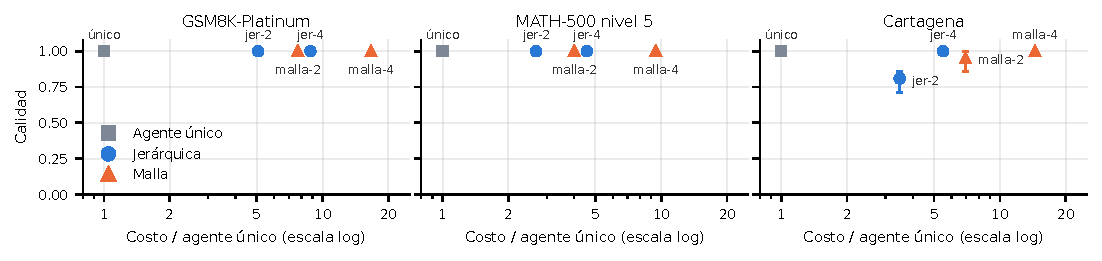
\includegraphics[width=\textwidth]{figs/calidad_vs_costo.pdf}
\caption{Calidad frente al costo relativo (escala logarítmica), con IC \textit{bootstrap} al 95\,\%. Cartagena se califica con la rúbrica aplicada a ciegas por un evaluador LLM, no humano.}
\label{fig:pareto}
\end{figure*}

\subsection{Coordinación y fallos}

\texttt{deepseek-flash} no tuvo ningún fallo técnico ni de coordinación en las 132 corridas de \textit{swarm}: todos los planes fueron JSON válido, todas las respuestas tuvieron el formato pedido y ninguna salida se truncó. En los dominios matemáticos la reina conservó la respuesta correcta en el 100\,\% de los casos. Los obreros sí se equivocaron: en 8 de las 40 corridas de MATH (y en 1 de las 80 de GSM8K) al menos un obrero dio un número incorrecto o sin formato; en 6 de los 8 casos fue el rol escéptico. En las 5 corridas de malla de MATH donde ocurrió, la revisión corrigió a todos los obreros equivocados. La redundancia funciona como mecanismo de corrección, pero solo repara errores que el agente único no cometió.

\subsection{Portabilidad}

El mismo código ejecutó un piloto de 20 corridas (108 llamadas) con \texttt{llama3.2:3b} y \texttt{qwen2.5:3b} en Ollama, en una GPU RTX 3050 de 4\,GB, cambiando solo la configuración. Esto muestra la agnosticidad de ingeniería. La Tabla~\ref{tab:fail} compara los modos de fallo y su correspondencia aproximada con MAST. Con una sola tarea por configuración, la comparación entre modelos es exploratoria: los modelos de 3B fallaron en el formato del plan y perdieron una respuesta correcta en la integración, modos que \texttt{deepseek-flash} no presentó. La latencia local no se compara con la de la API porque son infraestructuras distintas.

\begin{table}[t]
\centering
\caption{Fallos en corridas de \textit{swarm} y modo MAST más cercano \cite{cemri2025mast}}
\label{tab:fail}
\footnotesize
\setlength{\tabcolsep}{2.6pt}
\begin{tabular}{@{}L{2.3cm}cccL{1.85cm}@{}}
\toprule
Fallo & DeepSeek & Llama 3B & Qwen 3B & MAST \\
 & (132) & (8) & (8) & \\
\midrule
Plan JSON inválido & 0 & 2 & 0 & FM-1.1 (parcial) \\
Roles del plan & 0 & 1 & 0 & FM-1.1 (parcial) \\
Respuesta final truncada & 0 & 0 & 1 & --- \\
Reina pierde la correcta & 0 & 1 & 1 & FM-2.5/3.3 (candidato) \\
Contexto truncado & 0 & 0 & 0 & FM-1.4 (directo) \\
\bottomrule
\end{tabular}
\end{table}

\subsection{Hallazgos metodológicos}

Tres problemas habrían invalidado resultados sin instrumentación. Primero, en el piloto local un problema del GSM8K original tenía la etiqueta 2\,280 cuando la respuesta correcta es 2\,180; Qwen respondió 2\,180 en todas las configuraciones y se le contaba como error. GSM8K-Platinum corrige ese ítem \cite{vendrow2025platinum}. Segundo, Ollama trunca en silencio los \textit{prompts} que exceden su ventana: con la configuración por defecto, un \textit{prompt} de unos 9\,500 tokens se procesó como unos 2\,050. Por eso se fijó la ventana en 8\,192 tokens y se marcó como fallo toda llamada con más de 5 caracteres por token contado; el \textit{prompt} de 8\,129 tokens de la malla en MATH no habría cabido junto con la salida en esa ventana (con otro tokenizador la cifra es solo indicativa). Tercero, el juez LLM y la rúbrica dieron órdenes opuestos.

\section{Discusión}

Para \texttt{deepseek-flash}, la respuesta a la pregunta de investigación es negativa en las tres tareas: agregar agentes multiplicó el costo entre 2.7\x{} y 16.6\x{}, los tokens entre 4.1\x{} y 27.0\x{} y la latencia entre 2.3\x{} y 10.4\x{}, sin mejorar la calidad. La configuración más barata dentro del 95\,\% de la mejor calidad fue el agente único en los tres dominios. El resultado es coherente con el techo de capacidad de Kim et~al. \cite{kim2025scaling}: el modelo base ya resuelve estas tareas, así que la coordinación solo puede costar. La malla es la peor apuesta: con $n=4$ costó entre 1.9\x{} y 2.6\x{} lo que la jerárquica para la misma calidad, y su revisión crece con $n^2$.

El caso en que un \textit{swarm} podría pagar su costo es el contrario: tareas en que el agente único falla con frecuencia y de forma no correlacionada. La corrección interna observada en MATH indica que el mecanismo existe, pero la correlación de errores entre modelos \cite{kim2025correlated} y la amplificación medida en sistemas reales \cite{kim2025scaling} sugieren que la ganancia no está garantizada. La implicación práctica es medir primero al agente único y escalar la coordinación solo cuando la tarea lo justifique.

\section{Limitaciones y trabajo futuro}

Ambos dominios matemáticos quedaron en el techo, así que el estudio mide bien el costo de coordinar pero no puede mostrar ganancias de calidad. La matriz completa se ejecutó con un solo modelo; los dos modelos locales solo hicieron un piloto, y la agnosticidad empírica entre modelos queda sin probar. La tarea abierta es una sola, con tres repeticiones, y su calidad proviene de un único evaluador LLM a ciegas, no de evaluadores humanos. MATH usó una repetición por \textit{swarm} y se agregó después de ver el techo en GSM8K. La API no admite semilla, y GSM8K y MATH pueden estar en los datos de entrenamiento. Como trabajo futuro proponemos tareas en que el agente único falle (por ejemplo, problemas de competencia más difíciles), la matriz completa con varios modelos, evaluación humana con dos evaluadores y topologías podadas o adaptativas \cite{zhang2025agentprune,zhuge2024gptswarm}.

\section{Conclusiones}

Se construyó un orquestador reina--obreros que cambia de modelo y de dominio solo con configuración, y se midió con datos reales de uso cuánto cuesta coordinar. En tres dominios y 195 corridas, por USD~0.22, ni la jerárquica ni la malla mejoraron la calidad del agente único, y su costo creció entre 2.7\x{} y 16.6\x{}; la malla, más del doble de rápido que la jerárquica al aumentar $n$. Con un modelo capaz, la coordinación es un costo que solo se justifica en tareas que un único agente no resuelve.

\section*{Disponibilidad de código y datos}
El código, el cuaderno ejecutado, los registros de cada corrida y llamada, la evaluación ciega de Cartagena y los scripts que generan las tablas y figuras están en un repositorio público \cite{repo2026swarm}.

\begin{thebibliography}{99}

\bibitem{guo2024survey}
T.~Guo, X.~Chen, Y.~Wang, R.~Chang, S.~Pei, N.~V. Chawla, O.~Wiest, and X.~Zhang, ``Large language model based multi-agents: A survey of progress and challenges,'' arXiv:2402.01680, 2024.

\bibitem{wu2024autogen}
Q.~Wu, G.~Bansal, J.~Zhang \emph{et~al.}, ``AutoGen: Enabling next-gen LLM applications via multi-agent conversation,'' in \emph{Proc. Conf. Language Modeling (COLM)}, 2024. arXiv:2308.08155.

\bibitem{zhuge2024gptswarm}
M.~Zhuge, W.~Wang, L.~Kirsch, F.~Faccio, D.~Khizbullin, and J.~Schmidhuber, ``GPTSwarm: Language agents as optimizable graphs,'' in \emph{Proc. 41st Int. Conf. Machine Learning (ICML)}, PMLR 235, 2024.

\bibitem{ruflo}
ruvnet, ``Ruflo,'' repositorio de GitHub, 2026. \url{https://github.com/ruvnet/ruflo}

\bibitem{anthropic2025multiagent}
Anthropic, ``How we built our multi-agent research system,'' blog de ingeniería, 13 de junio de 2025. \url{https://www.anthropic.com/engineering/multi-agent-research-system}

\bibitem{cemri2025mast}
M.~Cemri, M.~Z. Pan, S.~Yang \emph{et~al.}, ``Why do multi-agent LLM systems fail?'' in \emph{Advances in Neural Information Processing Systems (NeurIPS), Datasets and Benchmarks Track}, 2025. arXiv:2503.13657.

\bibitem{kim2025scaling}
Y.~Kim, K.~Gu, C.~Park \emph{et~al.}, ``Towards a science of scaling agent systems,'' arXiv:2512.08296, 2025.

\bibitem{zhang2025agentprune}
G.~Zhang, Y.~Yue, Z.~Li, S.~Yun, G.~Wan, K.~Wang, D.~Cheng, J.~X. Yu, and T.~Chen, ``Cut the crap: An economical communication pipeline for LLM-based multi-agent systems,'' arXiv:2410.02506, 2024.

\bibitem{qian2025macnet}
C.~Qian, Z.~Xie, Y.~Wang \emph{et~al.}, ``Scaling large language model-based multi-agent collaboration,'' in \emph{Proc. Int. Conf. Learning Representations (ICLR)}, 2025.

\bibitem{li2024moreagents}
J.~Li, Q.~Zhang, Y.~Yu, Q.~Fu, and D.~Ye, ``More agents is all you need,'' \emph{Trans. Machine Learning Research (TMLR)}, 2024.

\bibitem{kim2025correlated}
E.~Kim, A.~Garg, K.~Peng, and N.~Garg, ``Correlated errors in large language models,'' in \emph{Proc. 42nd Int. Conf. Machine Learning (ICML)}, 2025.

\bibitem{kapoor2024agents}
S.~Kapoor, B.~Stroebl, Z.~S. Siegel, N.~Nadgir, and A.~Narayanan, ``AI agents that matter,'' arXiv:2407.01502, 2024.

\bibitem{deepseek2026pricing}
DeepSeek, ``Models \& pricing,'' documentación de la API, \url{https://api-docs.deepseek.com/quick_start/pricing}, consultado el 7 de octubre de 2026.

\bibitem{cobbe2021gsm8k}
K.~Cobbe, V.~Kosaraju, M.~Bavarian \emph{et~al.}, ``Training verifiers to solve math word problems,'' arXiv:2110.14168, 2021.

\bibitem{vendrow2025platinum}
J.~Vendrow, E.~Vendrow, S.~Beery, and A.~Madry, ``Do large language model benchmarks test reliability?'' arXiv:2502.03461, 2025.

\bibitem{lightman2024verify}
H.~Lightman, V.~Kosaraju, Y.~Burda \emph{et~al.}, ``Let's verify step by step,'' in \emph{Proc. Int. Conf. Learning Representations (ICLR)}, 2024.

\bibitem{hendrycks2021math}
D.~Hendrycks, C.~Burns, S.~Kadavath, A.~Arora, S.~Basart, E.~Tang, D.~Song, and J.~Steinhardt, ``Measuring mathematical problem solving with the MATH dataset,'' in \emph{Advances in Neural Information Processing Systems (NeurIPS), Datasets and Benchmarks Track}, 2021.

\bibitem{panickssery2024selfpref}
A.~Panickssery, S.~R. Bowman, and S.~Feng, ``LLM evaluators recognize and favor their own generations,'' in \emph{Advances in Neural Information Processing Systems (NeurIPS)}, 2024.

\bibitem{zheng2023judging}
L.~Zheng, W.-L. Chiang, Y.~Sheng \emph{et~al.}, ``Judging LLM-as-a-judge with MT-Bench and Chatbot Arena,'' in \emph{Advances in Neural Information Processing Systems (NeurIPS), Datasets and Benchmarks Track}, 2023.

\bibitem{mcnemar1947}
Q.~McNemar, ``Note on the sampling error of the difference between correlated proportions or percentages,'' \emph{Psychometrika}, vol.~12, no.~2, pp.~153--157, 1947.

\bibitem{cohen1960}
J.~Cohen, ``A coefficient of agreement for nominal scales,'' \emph{Educational and Psychological Measurement}, vol.~20, no.~1, pp.~37--46, 1960.

\bibitem{repo2026swarm}
J.~A. Mendoza Castro and E.~Gaviria Zambrano, ``swarm-llm-orchestrator,'' repositorio de GitHub, 2026. \url{https://github.com/EstebanGZam/swarm-llm-orchestrator}

\end{thebibliography}

\end{document}
